\chapter{Матрица упругости для слоистой среды}
\label{ch:layered_elasticity}

В случае однородной изотропной среды коэффициенты матрицы упругости $C_{i,j;k,l}$ могут быть найдены аналитическим способом из \eqref{eq:elasticity_kernel} путем интегрирования ядра $G(x,y;x',y')$ на элементе $\mathcal{A}_{i,j}$ \cite{Peir2008}
\begin{equation}
    \label{eq:homogeneous_matrix}
    C_{i,j;k,l} = -\frac{E'}{8\pi} \left[\frac{\sqrt{(x_i\!-\!x)^2 + (y_j\!-\!y)^2}}{(x_i\!-\!x)(y_j\!-\!y)} \right]_{x=x_k-\Delta x/2, y=y_l-\Delta y/2}^{x=x_k+\Delta x/2, y=y_l+\Delta y/2},
\end{equation}
где $[f]_{x=x_1, y=y_1}^{x=x_2, y=y_2} = f(x_1,y_1) - f(x_1,y_2) - f(x_2,y_1) + f(x_2,y_2)$.

В случае неоднородности по модулям упругости слоистой среды требуется численное построение матрицы упругости. Будем считать, что каждый слой есть упругая изотропная среда. Определяющие уравнения упругой изотропной среды задаются формулами
\begin{equation}
    \label{eq:equilibrium}
    \sigma_{ij,j} + f_j = 0,
\end{equation}
\begin{equation}		
    \sigma_{ij} = \lambda e_{kk}\delta_{ij} + 2G e_{ij},
    \label{eq:hooke_law}
\end{equation}
где $\lambda = \frac{E \nu}{(1+\nu)(1-2\nu)}$ и $ G = \frac{E}{2(1+\nu)} $.

Отделяя производные по $y$ от производных по $x, z$ в (\ref{eq:equilibrium}) и (\ref{eq:hooke_law}) \cite{Siebrits_Peirce_2002,Peirce2001TheSF,Peirce2001UniformAA}, получим
\begin{equation}
    \label{eq:separate}
    \partial_{y} T = \mathbb{A}T + F,
\end{equation}
где

\begin{equation}
    \label{eq:T}
    \begin{split}
        T &= \left[\sigma_{yy} \; \sigma_{xy} \; \sigma_{yz} \; u_{y} \; u_{x} \; u_{z}\right]^T, \\
        F &= \left[-f_y \; -f_x \; -f_z \; 0 \; 0 \; 0\right]^T,
    \end{split}
\end{equation}

и $\mathbb{A}$ -- дифференциальный оператор, который содержит производные только по $x$ и $z$
\begin{equation}
    \label{eq:A}
    \mathbb{A} = 
    \left[\begin{array}{cccccc}
        0                      & -\partial_x & -\partial_z & 0 & 0 & 0 \\
        -\frac{b}{a}\partial_x & 0           & 0 & 0 & \frac{b^2-a^2}{a}\partial_{xx} - \frac{f}{2}\partial_{zz} & \left( \frac{b^2-ab}{a} - \frac{f}{2} \right) \partial_{xz} \\
        -\frac{b}{a}\partial_z & 0           & 0 & 0 & \left( \frac{b^2-ab}{a} - \frac{f}{2} \right) \partial_{xz} & \frac{b^2-a^2}{a}\partial_{zz} - \frac{f}{2}\partial_{xx} \\
        \frac{1}{a}            & 0           & 0 & 0 & -\frac{b}{a}\partial_x & -\frac{b}{a}\partial_z \\
        0                      & \frac{2}{f} & 0 & -\partial_x & 0 & 0 \\
        0                      & 0           & \frac{2}{f} & -\partial_z & 0 & 0 
    \end{array}\right],
\end{equation}

где используются константы
\begin{align*}
    a   & = \lambda + 2G,                          & b   & = \lambda,                &     f & = 2G, \\
    l_2 & = \frac{\lambda + 3G}{\lambda + G},      & l_4 & = \frac{2G^2}{\lambda+G}, &   l_5 & = \frac{2G(\lambda + 2G)}{\lambda + G}, \\
    l_6 & = \frac{2G(2\lambda + 2G)}{\lambda + G}, & l_7 & = \frac{2\lambda G}{\lambda+G}
\end{align*}


Применим преобразование Фурье \eqref{eq:fourier_transform_2d} для (\ref{eq:separate}) по координатам $x$ и $z$
\begin{equation}
    \label{eq:FT_system}
    \partial_y \hat{T} = \hat{\mathbb{A}} \hat{T} + \hat{F},
\end{equation}
где
\begin{equation}
    \label{eq:FourierT}
    \begin{split}
        \hat{T} &= \left[\hat{\sigma}_{yy}/k \quad \hat{\tau}_s/k \quad \hat{u}_y \quad \hat{u}_s \quad  \hat{\tau}_t/k \quad  \hat{u}_t \right]^T, \\
        F &= \left[-\hat{f}_y \; -\hat{f}_s \; 0 \; 0 \; -\hat{f}_t \; 0\right]^T,
    \end{split}
\end{equation}
и оператор $\hat{\mathbb{A}}$
\begin{equation}
    \label{eq:FourierA}
    \hat{\mathbb{A}} = 
    \left[\begin{array}{cccccc}
        0 & -k & 0 & 0 & 0 & 0 \\
        \frac{b}{a}k & 0 & 0 & -\frac{b^2-a^2}{a}k^2 & 0 & 0 \\
        \frac{1}{a} & 0 & 0 & -\frac{b}{a}k & 0 & 0 \\
        0 & \frac{2}{f} & k & 0 & 0 & 0 \\
        0 & 0 & 0 & 0 & 0 & \frac{f}{2}k \\
        0 & 0 & 0 & 0 & \frac{2}{f} & 0 
    \end{array}\right].
\end{equation}

Здесь вводятся обозначения
\begin{equation}
    \label{eq:FT_special_variables}
    \begin{split}
        \hat{u}_s & = -i \frac{(m\hat{u}_x + n\hat{u}_z)}{k}, \\
        \hat{u}_t & = -i \frac{(n\hat{u}_x - m\hat{u}_z)}{k}, \\
        \hat{\tau}_s & = -i \frac{(m\hat{\sigma}_{xy} + n\hat{\sigma}_{yz})}{k}, \\
        \hat{\tau}_t & = -i \frac{(n\hat{\sigma}_{xy} - m\hat{\sigma}_{yz})}{k}. \\
    \end{split} 
\end{equation}

В случае $\hat{F} = 0$ система \eqref{eq:FT_system} является ОДУ и решение зависит от 6 свободных коэффициентов (\cite{Siebrits_Peirce_2002}, спектральные коэффициенты)
\begin{equation}
    \label{eq:fourier_solution}
    \left[
    \begin{array}{c}
        \hat{T}_s \\
        \hat{T}_t 
    \end{array}
    \right]
    =
    \left[
    \begin{array}{cc}
        Z_s & 0 \\
        0 & Z_t 
    \end{array}
    \right]
    \left[
    \begin{array}{c}
        A_s \\
        A_t 
    \end{array}
    \right]
\end{equation}

где используются обозначения
\begin{equation}
    \label{eq:FourierSeparateT}
    \hat{T}_s = \left[\hat{\sigma}_{yy}/k \quad \hat{\tau}_s/k \quad \hat{u}_y \quad \hat{u}_s \right]^T, \qquad 
    \hat{T}_t = \left[ \hat{\tau}_t/k \quad  \hat{u}_t \right]^T.
\end{equation}

Матрицы $Z_s$ и $Z_t$ имеют вид
\begin{equation}
    \label{eq:FourierSeparateA}
    \begin{split}
    Z_s & = 
    \left[
    \begin{array}{cccc}
        -fe^{-ky} & (l_4-fky)e^{-ky} & fe^{ky} & (l_4+fky)e^{ky} \\
        -fe^{-ky} & (l_5-fky)e^{-ky} & -fe^{ky} & -(l_5+fky)e^{ky} \\
        e^{-ky} & kye^{-ky} & e^{ky} & kye^{ky} \\
        e^{-ky} & (ky-l_2)e^{-ky} & -e^{ky} & -(ky+l_2)e^{ky} \\
    \end{array}
    \right],
    \\
    Z_t & = 
    \left[
    \begin{array}{cc}
        -\frac{f}{2}e^{-ky} & \frac{f}{2}e^{ky} \\
        e^{-ky} & e^{ky}
    \end{array}
    \right].
    \end{split}
\end{equation}

Из \eqref{eq:fourier_solution} получаем связь между спектральными коэффициентами и значениями смещений и напряжений на границе слоя
\begin{equation}
    \label{eq:As}
    \left[
    \begin{array}{c}
    A^{j}_{1}(k) \\
    A^{j}_{2}(k)\\
    A^{j}_{3}(k) \\
    A^{j}_{4}(k)
    \end{array}
    \right]
    = \frac{1}{2l^j_5}
    \left[
    \begin{array}{cccc}
        -l^j_2 & 0 & l^j_5 & -l^j_4 \\
        -1 & 1 & f^j & -f^j \\
        l^j_2 & 0 & l^j_5 & l^j_4 \\
        -1 & -1 & -f^j & -f^j
    \end{array}
    \right]
    \left[
    \begin{array}{c}
    \hat{\sigma}^{j}_{yy}(y=y_j)/k \\
    \hat{\tau}^{j}_{s}(y=y_j)/k\\
    \hat{u}^{j}_{y}(y=y_j) \\
    \hat{u}^{j}_{s}(y=y_j) 
    \end{array}
    \right],
\end{equation}

\begin{equation}
    \label{eq:At}
    \left[
    \begin{array}{c}
        A^{j}_{5}(k) \\
        A^{j}_{6}(k)
    \end{array}
    \right]
    = \frac{1}{2l^j_5}
    \left[
    \begin{array}{cc}
        -\frac{1}{f^j} & \frac{1}{2} \\
        \frac{1}{f^j} & \frac{1}{2}
    \end{array}
    \right]
    \left[
    \begin{array}{c}
    \hat{\tau}^{j}_{t}(y=y_j)/k\\
    \hat{u}^{j}_{t}(y=y_j) 
    \end{array}
    \right].
\end{equation}

\begin{figure}[htbp]
    \centering
    \begin{subfigure}[b]{0.45\textwidth}
        \centering
        \caption{Условие точечного разрыва смещений}
        \label{fig:DD_point}
        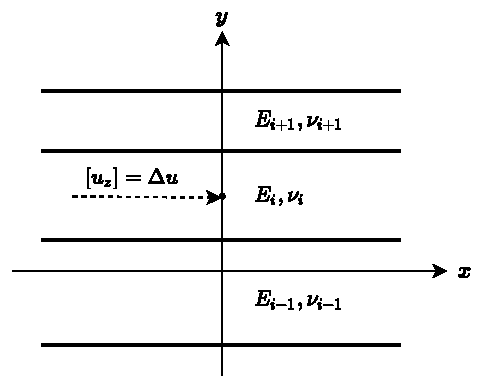
\includegraphics[width=\textwidth]{DD_point.pdf}
    \end{subfigure}
    \hfill 
    \begin{subfigure}[b]{0.45\textwidth}
        \centering
        \caption{Введение дополнительной границы}
        \label{fig:pseudointerface}
        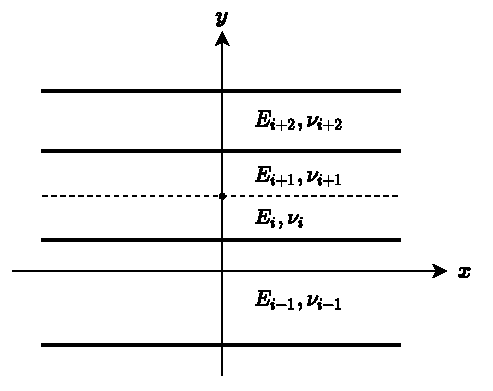
\includegraphics[width=\textwidth]{DD_point2.pdf}
    \end{subfigure}
    \caption{Введение псевдо-границы}
    \label{fig:Pseudointerface}
\end{figure}

Введём псевдо-границу (рисунок~\ref{fig:pseudointerface}) вдоль точки, в которой ставится условие разрыва смещений (рисунок~\ref{fig:DD_point}). Тогда $u_{z-0} - u_{z+0} = \Delta u$ может быть представлена в виде скачка смещения и напряжений на границе раздела слоев
\begin{multline}
    \label{eq:jump_condition}
    \left[ \hat{T} \right] = \hat{T}(y-0) - \hat{T}(y+0) = 
    \left[ \begin{array}{c} 
        0 \\ \frac{\Delta u(b^2 - a^2)}{a} \\ \frac{\Delta ub}{a} \\ 0 \\ 0 \\ 0 
    \end{array} \right]
    +
    \frac{m^2}{m^2+n^2} \left[ \begin{array}{c} 
        0 \\ \Delta u(a-b) \\ 0 \\ 0 \\ 0 \\ 0 
    \end{array} \right]
    + \\ +
    \frac{mn}{m^2+n^2} \left[ \begin{array}{c} 
        0 \\ 0 \\ 0 \\ 0 \\ \Delta u(a-b) \\ 0 
    \end{array} \right].
\end{multline}

Таким образом, мы получаем системы ОДУ для каждого слоя, связанные условиями неразрывности или \eqref{eq:jump_condition} на границе. Из этих соотношений можно составить уравнения для определения компонент вектора смещения и напряжений на границе раздела слоев
\begin{equation}
    \label{eq:coupled_t-system}
    A_t^i \hat{\tau}_t^{i-1} + C_t^i \hat{\tau}_t^{i} + B_t^i \hat{\tau}_t^{i+1} = D_t^i,
\end{equation}
для t-системы и 
\begin{equation}
    \label{eq:coupled_s-system}
    \textbf{A}_s^i \left[
        \begin{array}{c}
            \hat{\sigma}_{yy}^{i-1} \\
            \hat{\tau}_s^{i-1}
        \end{array}\right] +
    \textbf{C}_s^i \left[
        \begin{array}{c}
            \hat{\sigma}_{yy}^{i} \\
            \hat{\tau}_s^{i}
        \end{array}\right] + 
    \textbf{B}_s^i \left[
        \begin{array}{c}
            \hat{\sigma}_{yy}^{i+1} \\
            \hat{\tau}_s^{i+1}
        \end{array}\right]
    = \textbf{D}_s^i,
\end{equation}
для s-системы. Значения матриц в \eqref{eq:coupled_t-system} и \eqref{eq:coupled_s-system} приведены в приложении~\ref{app:coupled_systems}.

Решая \eqref{eq:coupled_t-system} и \eqref{eq:coupled_s-system}, находим спектральные коэффициенты для каждого слоя из \eqref{eq:As} и \eqref{eq:At}. Окончательно, используя закон Гука \eqref{eq:hooke_law} и \eqref{eq:fourier_solution}, получим
\begin{multline}
    \label{eq:fourier_sigmazz}
    \hat{\sigma}^j_{zz}(y)/k = f\frac{n^2}{k^2}e^{-ky}A^j_1(k)
    - \left(l_6\frac{n^2}{k^2}+l_7\frac{m^2}{k^2}-f\frac{n^2}{k^2}ky \right)e^{-ky}A^j_2(k) - \\
    - f\frac{n^2}{k^2}e^{ky}A^j_3(k)
    - \left(l_6\frac{n^2}{k^2}+l_7\frac{m^2}{k^2}+f\frac{n^2}{k^2}ky \right)e^{ky}A^j_4(k) - \\
    - f\frac{mn}{k^2}e^{-ky}A^j_5(k)
    - f\frac{mn}{k^2}e^{ky}A^j_6(k).
\end{multline}
Применяя обратное дискретное преобразование Фурье \eqref{eq:DFT}, находим $\sigma_{zz}(y,x',y')$.

Условие \eqref{eq:jump_condition} является сингулярным в точке, в которой ставится условие разрыва смещений. Используя линейность определяющих уравнений \eqref{eq:equilibrium} и \eqref{eq:hooke_law}, можем представить ядро $G(x,y;x',y')$ для слоистой среды в виде
\begin{equation}
    G(x,y;x',y') = G_\text{hom}(x,y;x',y') + G'(x,y;x',y'),
\end{equation} 
где $G_\text{hom}(x,y;x',y')$ получается из \eqref{eq:elasticity_kernel} с учетом $E'=E'(y)$. Таким образом, удается избавится от сингулярности в условие \eqref{eq:jump_condition} и можем записать
\begin{equation}
    \label{eq:heterogeneous_kernel}
    G'(x,y;x',y') = -\Delta \sigma_{zz}(y, x', y'),
\end{equation}
где $\Delta \sigma_{zz}(y, x', y')$ находится из \eqref{eq:fourier_sigmazz}.
